

\documentclass[a4paper,english]{lipics-v2016}
\usepackage{microtype}

%% This is our standard package for code formatting:
\usepackage{listings}
\usepackage{amsmath}
\usepackage{amsthm}
\usepackage{hyperref}
\usepackage{graphicx}
% \usepackage{mathabx}
% \usepackage{mathpartir}

\usepackage[noabbrev]{cleveref}
\usepackage{enumitem}

\usepackage{wrapfig}

\usepackage[labelformat=simple]{subcaption}

%Re-formatting figure captions to make subfigures look right.
\newcommand{\myhrule}{ \leaders\hrule width 0pt height .33pt \hfill }
\renewcommand{\myhrule}{\hrulefill}

\DeclareCaptionFormat{ruled}{\myhrule \\ #1#2#3}
\DeclareCaptionFormat{plain}{#1#2#3}

\captionsetup[figure]{format=ruled}
\captionsetup[subfigure]{format=plain}

\newcommand{\treecomp}{Gibbon compiler{}}

%% Traversal effects:
\newcommand{\travarr}[1]{\xrightarrow{#1}}
% \newcommand{\arr}[3]{\ensuremath{{#1} \xrightarrow{\overrightarrow{#2}} {#3}}}
% \newcommand{\arr}[3]{\ensuremath{{#1} \xrightarrow{trav({#2})} {#3}}}
\newcommand{\arr}[3]{\ensuremath{{#1} \travarr{#2} {#3}}}
% $\xrightarrow[world]{hello}$



\renewcommand{\thesubfigure}{(\alph{subfigure})}

\newcommand{\fresh}[1]{\ensuremath{#1}}
\newcommand{\fixed}[1]{\ensuremath{\texttt{#1}}}

\newcommand{\freshA}{\fresh{\alpha}}
\newcommand{\freshB}{\fresh{\beta}}
\newcommand{\locend}[1]{\ensuremath{\overline{#1}}}

\newif\ifcurly
\curlytrue % Comment to deactivate.


%----------------------------------------
%% \usepackage[colorinlistoftodos,prependcaption,textsize=tiny]{todonotes}
%% \usepackage{xargs}
%% \newcommandx{\unsure}[2][1=]{\todo[linecolor=red,backgroundcolor=red!25,bordercolor=red,#1]{#2}}
%% \newcommandx{\info}[2][1=]{\todo[linecolor=OliveGreen,backgroundcolor=OliveGreen!25,bordercolor=OliveGreen,#1]{#2}}
%% \newcommandx{\change}[2][1=]{\todo[linecolor=blue,backgroundcolor=blue!25,bordercolor=blue,#1]{#2}}
%% \newcommandx{\inconsistent}[2][1=]{\todo[linecolor=blue,backgroundcolor=blue!25,bordercolor=red,#1]{#2}}
%% \newcommandx{\improvement}[2][1=]{\todo[linecolor=Plum,backgroundcolor=Plum!25,bordercolor=Plum,#1]{#2}}
%% \newcommandx{\resolved}[2][1=]{\todo[linecolor=OliveGreen,backgroundcolor=OliveGreen!25,bordercolor=OliveGreen,#1]{#2}} % use this to mark a resolved question
%% \newcommandx{\thiswillnotshow}[2][1=]{\todo[disable,#1]{#2}} % will replace \resolved in the final document
% ----------------------------------------


% Tweak width of margin notes for this documentclass:
\setlength{\marginparwidth}{1.75cm}
% Copy this if needed to customize:
\input{./bibs/latex_templates/editingmarks}

% If we are using Haskell code in this paper:

\usepackage{upquote}
\usepackage{listings}
\usepackage[usenames,dvipsnames]{xcolor}

\definecolor{darkgreen}{rgb}{0,0.5,0}
\definecolor{darkred}{rgb}{0.5,0,0}

% Define the language styles we will use
%
\lstset{%
    frame=none,
    rulecolor={\color[gray]{0.7}},
    numbers=none,
    basicstyle=\ttfamily,        
%    basicstyle=\smallsize\ttfamily,    
%    basicstyle=\footnotesize\ttfamily,
%    basicstyle=\scriptsize\ttfamily,
%    basicstyle=\Largesize\ttfamily,        
    numberstyle=\color{Gray}\tiny\it,
    commentstyle=\color{MidnightBlue}\it,
    stringstyle=\color{Maroon},
    keywordstyle=[1],
    keywordstyle=[2]\color{ForestGreen},
    keywordstyle=[3]\color{Bittersweet},
    keywordstyle=[4]\color{RoyalPurple},
    captionpos=b,
    aboveskip=1\medskipamount,
    xleftmargin=0.5\parindent,
    xrightmargin=0.5\parindent,
    flexiblecolumns=false,
%   basewidth={0.5em,0.45em},           % default {0.6,0.45}
%    escapechar={\%},
    escapechar={\@},
    mathescape=true,
    texcl=true                          % tex comment lines
}

\lstloadlanguages{Haskell}
\lstdefinestyle{haskell}{%
    language=Haskell,
    upquote=true,
    basicstyle=\ttfamily,        
    deletekeywords={case,class,data,default,deriving,do,in,instance,let,of,type,where,IO,ST,STM,read},
%    morekeywords={[1]read,write,finish},
    morekeywords={[2]class,data,default,deriving,family,instance,type,where},
    morekeywords={[3]in,let,case,of,do,switch},
    morekeywords={[4]IORef,IO,ST,STM,Symbol},
    literate=
        {\\}{{$\lambda$}}1
        {\\\\}{{\char`\\\char`\\}}1
        {>->}{>->}3
        {>>=}{>>=}3
        {->}{{$\rightarrow$}}2
        {>=}{{$\geq$}}2
        {<-}{{$\leftarrow$}}2
        {<=}{{$\leq$}}2
        {=>}{{$\Rightarrow$}}2
        {|}{{$\mid$}}1
        {forall}{{$\forall$}}1
        {exists}{{$\exists$}}1
        {...}{{$\cdots$}}3
%       {`}{{\`{}}}1
%       {\ .}{{$\circ$}}2
%       {\ .\ }{{$\circ$}}2
%
%    deletekeywords={insert},
%    deletekeywords={map,sort,zipWith,replicate,Num,Char,Bool,Array,Int,Double
%                   ,sqrt,not,filter,IO,Maybe,Either,quot,scanl,scanr,reverse,fst,id},
%    literate=
%        {+}{{$+$}}1
%        {/}{{$/$}}1
%        {*}{{$*$}}1
%        % {=}{{$=$}}1
%        {>}{{$>$}}1 {<}{{$<$}}1
%        {\\}{{$\lambda$}}1
%        {\\\\}{{\char`\\\char`\\}}1
%        {->}{{$\rightarrow\;$}}2
%        {>=}{{$\geq$}}2
%        {<-}{{$\leftarrow\;$}}2
%        {<=}{{$\leq$}}2
%        {=>}{{$\Rightarrow\;$}}2
%        {\ .}{{$\circ$}}2
%        {\ .\ }{{$\circ$}}2
%        {>>}{{>>}}2
%        {>>=}{{>>=}}2
%        {=<<}{{=<<}}2
%        {|}{{$\mid$}}1
%        {dotdotdot}{{$\ldots$}}3
}

\lstdefinestyle{inline}{%
    style=haskell,
%    basicstyle=\footnotesize\ttfamily,
    basicstyle=\ttfamily,
    %% keywordstyle=[1],
    %% keywordstyle=[2],
    %% keywordstyle=[3],
    %% keywordstyle=[4],
    literate=
        {\\}{{$\lambda$}}1
        {\\\\}{{\char`\\\char`\\}}1
        {>->}{>->}3
        {>>=}{>>=}3
        {->}{{$\rightarrow$\space}}3    % include forced space
        {>=}{{$\geq$}}2
        {<-}{{$\leftarrow$}}2
        {<=}{{$\leq$}}2
        {=>}{{$\Rightarrow$}}2
        {|}{{$\mid$}}1
%        {~}{{$\sim$}}1
        {forall}{{$\forall$}}1
        {exists}{{$\exists$}}1
        {...}{{$\cdots$}}3
}

\lstnewenvironment{code}
    {\lstset{style=haskell}%
      \csname lst@SetFirstLabel\endcsname}
    {\csname lst@SaveFirstLabel\endcsname}
    {}

% Default all listings to Haskell style
\lstset{style=haskell}

% \newcommand{\inl}[1]{\lstinline[style=inline];#1;}
\newcommand{\il}[1]{\lstinline[style=inline];#1;}

\newcommand{\makeatcode}{\lstMakeShortInline[style=inline]@}
\newcommand{\makeatchar}{\lstDeleteShortInline@}


% Sometimes we have extra short-cuts:
% \input{macro-defs}

% Sometimes we factor large figures into commands in a separate file:
% \input{figures}



%\special{papersize=8.5in,11in}
%\setlength{\pdfpageheight}{\paperheight}
%\setlength{\pdfpagewidth}{\paperwidth}

%\conferenceinfo{CONF 'yy}{Month d--d, 20yy, City, ST, Country}
%\copyrightyear{20yy}
%\copyrightdata{978-1-nnnn-nnnn-n/yy/mm}
%\copyrightdoi{nnnnnnn.nnnnnnn}

% Uncomment the publication rights you want to use.
%\publicationrights{transferred}
%\publicationrights{licensed}     % this is the default
%\publicationrights{author-pays}

%\titlebanner{banner above paper title}        % These are ignored unless
%\preprintfooter{short description of paper}   % 'preprint' option specified.

\newcommand{\treelang}{Gibbon} % NEED NAME

\title{Compiling tree transforms to operate on packed representations}
% \subtitle{Faster compiler passes, parallelization ready}

%\authorinfo{Name1}
%           {Affiliation1}
%           {Email1}
%\authorinfo{Name2\and Name3}
%           {Affiliation2/3}
%           {Email2/3}

\author[1]{John Q. Open}
\author[2]{Joan R. Access}
\affil[1]{Dummy University Computing Laboratory, Address/City, Country\\
  \texttt{open@dummyuniversity.org}}
\affil[2]{Department of Informatics, Dummy College, Address/City, Country\\
  \texttt{access@dummycollege.org}}
\Copyright{John Q. Open and Joan R. Access}%mandatory, please use full first names. LIPIcs license is "CC-BY";  http://creativecommons.org/licenses/by/3.0/
\subjclass{Dummy classification -- please refer to \url{http://www.acm.org/about/class/ccs98-html}}% mandatory: Please choose ACM 1998 classifications from http://www.acm.org/about/class/ccs98-html . E.g., cite as "F.1.1 Models of Computation". 
\keywords{Dummy keyword -- please provide 1--5 keywords}% mandatory: Please provide 1-5 keywords
%Editor-only macros:: begin (do not touch as author)%%%%%%%%%%%%%%%%%%%%%%%%%%%%%%%%%%

\begin{document}

\maketitle

\begin{abstract}
When written idiomatically in most programming languages, programs that traverse
and construct trees operate over pointer-based data structures, with one heap
object per-leaf and node.  While this may seem tautological, we show that common
tree traversals---found in compiler passes, space-partitioning trees, and
elsewhere---can instead be automatically compiled to operate on pointer-free
pre-order serializations of trees.  On current x86 architectures such programs
can run up to several times faster than their pointer-based counterparts.

We present a prototype compiler for a small first-order, purely functional
language of tree traversals.  The output language includes mutable cursors into
input and output buffers for packed data.  We propose a compilation technique
with an effect system for capturing traversal behavior, combined with a
lightweight analysis inferring data flow, and a program synthesis step for
creating missing traversals.
  
\end{abstract}

%\category{CR-number}{subcategory}{third-level}

% general terms are not compulsory anymore,
% you may leave them out
%\terms
%term1, term2

%\keywords
%keyword1, keyword2

% ================================================================================
\section{Introduction}
% ================================================================================

\rn{This is an example peanut-gallery comment.}

Programs that traverse and construct trees are a niche, but an important one,
including compiler passes, HTML DOM, and particle simulations with
space-partitioning trees.
%
Yet there is almost no diversity in how modern programming languages and
compilers represent trees and their traversals, so the matter would seem to be
settled.
% In the traditional representation,
Each node of the tree is a heap object, followed by fields for child nodes or
leaf values.  This representation hasn't changed since the dawn of computing and
is shared across source languages with quite different type
systems---whether algebraic datatypes or class hierarchies, either statically or
dynamically typed.  The only deviations from this consensus are found within
limited high-performance scenarios where complete trees can be laid out using
address arithmetic with no intermediate nodes \cite{hpc-trees}.

But perhaps the consensus was premature?  In numerical computing it is an axiom
that you cannot treat the numbers in a matrix as individual heap objects.
Rather, the emphasis is on bulk efficiency.  Likewise, many tree traversals
process trees in bulk, reading or writing them in one pass.  On such workloads,
traditional tree representations are not favored by current trends in computer
architecture.  Pointer chasing implies randomized memory access patterns.
%
While previous work addresses spatial locality for tree data\cite{Chilimbi1999},
%
much memory is still wasted both in pointers themselves and in tags on nodes
(e.g. distinguishing ``interior'' vs ``leaf'' objects).  For example, a C
compiler uses 96 bytes
%
%% \rn{Double check that for alignment the C compiler is sacrificing a word for the
%% one byte tag field.} 
%
of memory to represent the tree shown in Figure~\ref{fig:intro-tree-unpacked}. On the other hand, if we are sending the tree over the network, we would naturally use a more compact form in serializing it, as shown in Figure~\ref{fig:intro-tree-packed}.   
In the latter version, we use the same 24 bytes for the data in the leaves, but only 5 bytes for the
spine (capturing the ``tags'' of the 5 nodes in the tree), rather than 72.  Further, a tree traversal processing this memory
representation follows a precisely linear memory access pattern, because the
data is already laid out in a preorder traversal.
%
On architectures with inexpensive unaligned access, such as modern x86, this is
a desirable in-memory representation as well as a serialization format.

\begin{figure}
  \begin{subfigure}[t]{\linewidth}
    \centering
    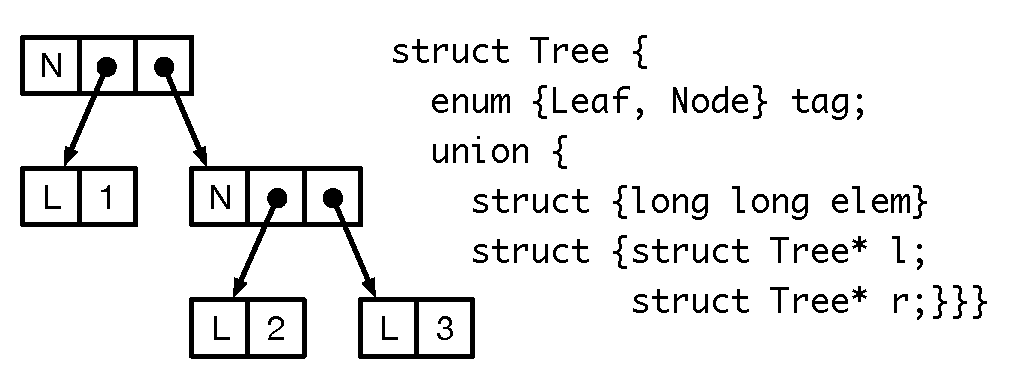
\includegraphics[scale=0.5]{figs/intro-tree-unpacked}
    \caption{Standard representation of a tree structure in C}
    \label{fig:intro-tree-unpacked}
  \end{subfigure}
  \begin{subfigure}[t]{\linewidth}
    \centering
    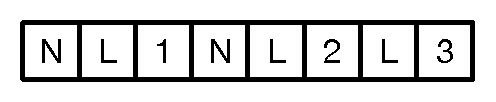
\includegraphics[scale=0.5]{figs/intro-tree-packed}
    \caption{Serialized version of the same tree}
    \label{fig:intro-tree-packed}    
  \end{subfigure}
  \caption{Standard and serialized representations of trees}
\end{figure}

% \begin{figure}
%% \begin{figure}
%% %\begin{wrapfigure}{r}{0.5\textwidth} 
%% \Red{PICTURE HERE:  possibly with wrapfig.}
% \begin{verbatim}
%  [N|.|.]          struct Tree {
%     /  \           enum { Leaf, Node } tag;
% [L 1]  [N|.|.]     union { 
%          /   \      struct { long long elem; };
%       [L 2] [L 3]   struct { struct Tree* l;
%                              struct Tree* r; }}}
% \end{verbatim}

%%   \caption{Traditional, pointer-based tree layout.}
%% \end{figure}
%\end{wrapfigure}
% \begin{verbatim}
%   [N L 1  N L 2  L 3 ]
% \end{verbatim}
% \end{figure}

Indeed, if we can compile programs to operate directly on this serialization, we
follow a precedent of using serialization formats jointly as in memory formats.
For example, Cap'N Proto \cite{capnproto} makes it ergonomic for C++ code to operate directly
on the Protobuf serialization format in memory.  Likewise ``data baking''
\cite{data-baking} is an established practice in video games---caching assets on
disk in a format that allows them to be \il{mmap}'d into memory and used
without further conversion.  As a general example of this capability, the
Glasgow Haskell Compiler (GHC) recently added the capability to store any closed
subgraph of the heap as a {\em Compact Normal Form} (CNF) \cite{cnf-icfp15}---a
contiguous memory region that is treated as a kind of ``super object'', never
traced by the GC and collected only when there are no pointers into any of the
sub-parts of the CNF.

The packed tree format above is precisely a dense encoding of a CNF---a
transitive closure of heap objects with no escaping pointers, in this case, no
pointers {\em at all}.  But unlike GHC's CNF support, which uses regular heap
objects, colocated together, the dense tree format {\em requires a complete
rearrangement of the compiled code that operates on the data}.

% Shall we acronymize it?
% DTF - dense tree form, or dense tree format
% PTF - packed tree form
% DTP - dense tree packing

In this paper, we take a first step towards compiler support for transparently
packing tree datatypes {\em without} changing the source program.  We make the
following contributions:

\newcommand{\calculus}{$\lambda^D_T$} % uh, Dense Tree?

\begin{itemize}
\item We use a small core language, \calculus{}, to formalize a transformation
  on programs with threes that creates an output program that operates only on
  pointers in the serialized representation.  This involves a small program
  synthesis step, and we show how the program synthesis and the selection of
  data structure shape go benefit from co-optimization.
  
\item We demonstrate that a prototype language implementation based on this
  transformation can compile a range of tree transforms to be several times
  faster than existing techniques~\cref{sec:eval-compiler}.
  
\item We show that the principle of packed-tree traversals works across a
  variety of language implementations, by benchmarking handwritten packed-tree
  programs~\cref{sec:eval-shootout}.
  
\item We show that not only do tree traversals become faster, but that their
  {\em potential parallel speedup}, increases as well \cref{sec:eval-parallel}.
\end{itemize}


% ================================================================================
% \section{Motivating Example}
\section{Background and Example}
% ================================================================================

While our main emphasis in this paper is on accelerating compiler passes, here
we continue with our simple example from the introduction: binary trees with
integer leaves.
In a language with algebraic datatypes,
% In a strongly typed functional language,
a recursive walk on
the tree would typically use pattern matching:

\ifcurly
% [language=python]
\begin{code}[language=c]
type Tree = Leaf(Int) | Node(Tree,Tree);

fun add1(t) {
  match(t) {
    Leaf(n):   return Leaf(n+1);
    Node(x,y): return Node(add1(x),add1(y));
  }}
\end{code}
\else
\begin{code}
 data Tree = Leaf Int | Node Tree Tree
  
 add1 t =
  case t of
    Leaf n   -> Leaf (n+1)
    Node x y -> Node (add1 x) (add1 y)
\end{code}
\fi

In fact, the small, first-order, purely functional language of tree traversals
we consider this paper is already a subset of most existing languages.
The above program is not substantially different in C, Haskell, ML, Scala,
Swift, Rust, etc.  Only the details of switching on sum types (tagged unions) differ.

The first problem for tree-walks such as this is memory management.  \il{add1}
can easy become a malloc or garbage collector benchmark.  For instance, the
following C code is over twice as slow as the same implementation in Java or a
good functional compiler:

\begin{code}[language=c]
  Tree* add1(Tree* t) {
    Tree* tout = (Tree*)malloc(sizeof(Tree));
    tout->tag = t->tag;
    if (t->tag == Leaf) {
      tout->elem = t->elem + 1;
    } else {
      tout->l = add1(t->l);
      tout->r = add1(t->r);
    }
    return tout;
  }
\end{code}

But even if we assume optimal layout, bump-pointer allocation, and {\em no
  header objects}---even if we go further and enable \il{__packed__} attribute
for our structs to save tag space---the performance of the above code is still
several times below what is achievable.  The main observation of this paper is
that bulk tree walks are efficient if done directly on pre-order serialization
of the tree, and that it is possible to automate the translation of recursive
functions, such as @add1@ above, into code that directly manipulates data
buffers containing serialized trees.

For our simple example, this buffer passing code isn't complicated:
%
\begin{code}[language=c]
char* add1(char* tin, char* tout) {
  if (*tin == Leaf) {
    *tout = Leaf;
    tin++; tout++;
    *(int*)tout = *(int*)tin;
    return (tin + sizeof(int));
  } else {
    *tout = Node;
    tin++; tout++;
    char* t2 = add1Tree(tin,tout);
    tout += (t2 - t);
    return add1Tree(t2,tout);
  }
}
\end{code}
%
Yet this approach cannot scale--it quickly becomes tedious and error prone.
Clearly, no one would use a technique like this for building a compiler!

The above program is similar to the output produced by the prototype compiler we
describe in this paper.  We refer to the input and output pointers as {\em
  cursors}, and one of the primary jobs of the compiler is automatic cursor
insertion.

%% \note{Yet, code performing raw manipulation of a pointer into a byte buffer
%%   containing a serialized tree is extremely error prone and tedious to write.
%%   It certainly is inappropriate for writing compilers, which contain reams and
%%   reams of tree-walking code.}

\subsection{Challenges and Limitations}

\note{Rightmost vs leftmost}


\ifcurly
\begin{code}[language=c]
fun left(t) {
  match(t) {
    Leaf(n):   return n;
    Node(x,_): return left(x);
  }}
fun right(t) {
  match(t) {
    Leaf(n):   return n;
    Node(_,y): return right(y);
  }}
\end{code}
\else
\begin{code}
 left t = case t of
            Leaf n   -> n
            Node x _ -> left x
 right t = case t of
             Leaf n   -> n
             Node _ y -> right y
\end{code}
\fi


\subsection{Related Work}

\rn{Milind, some of the related work was going to go up here?}

One line of closely related work focuses on managing data layout in trees and
other data structures to promote spatial
locality~\cite{Chilimbi1999,Chilimbi1999b,Truong1998,Lattner2005,Chilimbi1999a},
by modifying garbage collection to co-locate objects~\cite{Chilimbi1999a},
modifying memory allocators to proactively place objects with similar access
patterns together~\cite{Lattner2005,Chilimbi1999}, or to modify the internal
layout of objects to place hot fields near each other~\cite{Chilimbi1999b}.
These approaches attempt to ``pack'' data together, using various techniques,
into cache lines to improve spatial locality, and hence have some resemblance
to our packed representations, which gain some performance benefits from
packing tree data into a compact format that promotes spatial locality.

Perhaps the most closely related of these is Chilimbi et al.'s {\em cache
conscious structure layout}~\cite{Chilimbi1999}. They propose a
cache-conscious data placement scheme where, given a traversal function,
tree-structured data will be laid out in memory in a {\em clustered} manner:
nodes from small subtrees will be placed on single cache lines. By matching
the tree layout to a specified traversal order, spatial locality is improved
when the tree is traversed in that order. A key difference between our packed
representation and Chilimbi et al.'s work is that this work focused on object
layout, without changing the internal {\em representation} of the objects.
Leaving the object representation of tree nodes the same allows code that
manipulates the objects to remain the same, but incurs costs: there is no
opportunity to reduce the space or instruction overhead incurred by pointers
linking nodes in the tree (see Figure~\ref{fig:intro-fig}), as exploiting that
opportunity requires code transformation. Most of the aforementioned spatial
locality work makes the same tradeoff.

One exception is Chilimbi et al.'s work on {\em automatic structure
splitting}~\cite{Chilimbi1999b}, where objects are transformed into split
representations, allowing hot fields from multiple objects to be co-located on
a single cache line while those objects' cold fields are placed elsewhere.
Because this layout optimization changes the internal representation of the
object, Chilimbi et al. develop a compiler pass that automatically transforms
code to work with the split representation. The transformations for structure
splitting concern how to access object fields, and hence, unlike our work, do
not require deeper transformations to remove the pointer dereferences inherent
in traversing linked data structures.


% ================================================================================
\section{The \treelang{} Language}
% ================================================================================

\note{Informal overview of language}

To demonstrate the compilation technique we are presenting, we present
$\treelang{}$, a typed programming language that is simple enough to
present briefly in a paper, and featureful enough to express some
interesting programs, such as common compiler passes.

Programs consist of a series of data type declarations and function
declarations. Similar to most functional programming languages,
programmers may define \emph{algebraic data types}, and dispatch on
them with a \texttt{match} language form (called \texttt{case} or
\texttt{switch} in some languages).
%% For example, a data type for peano
%% numbers would have two cases: zero and successor.

\note{We already gave an example of a program in Gibbon earlier...
  probably only need one, unless we're doing something different here}

%% \begin{code}[language=haskell]
%% type Nat = Zero | Suc(Nat);
%% \end{code}

%% For simplicity, $\treelang{}$ is a first-order language, so all
%% functions are defined at the top level.

%% \begin{code}[language=haskell]
%% fun trav(x) {
%%   match(x) {
%%     Zero: return 0;
%%     Suc(n): return 1 + trav(n);
%% }}
%% \end{code}

In addition to algebraic data types and various numerical types, $\treelang{}$ supports
general purpose persistent dictionaries, which are useful for implementing compiler
passes in a functional style.

\note{Show an example of using a dictionary? Or just give the types?}

\note{Describe the Racket front-end and how it works.}

% ================================================================================
\section{Formal Language}
% ================================================================================


\note{The calculus, plus the core lowering transforms in figures.}

%% We present two languages: L1, a simple purely functional, first-order programming
%% language with sum and product types; and L2, an imperative programming language
%% with mutable arrays and pointer arithmetic, as well as a type-and-effect system.


\newcommand{\gramdef}{\; ::= \;}
\newcommand{\gramor}{\; | \;}
\newcommand{\PROG}{\keywd{prog}}
\newcommand{\EXPR}{\keywd{e}}
% \newcommand{\PRIM}{\keywd{\rho}}
\newcommand{\PRIM}{\odot}
\newcommand{\TYP}{\keywd{\tau}}
\newcommand{\ARROW}{\rightarrow}
\newcommand{\DD}{\keywd{dd}}
\newcommand{\VD}{\keywd{vd}}
\newcommand{\FD}{\keywd{fd}}
\newcommand{\TC}{\keywd{T}}
\newcommand{\DC}{\keywd{K}}

\ifcurly
\newcommand{\DATA}{\gramwd{type}}
\else
\newcommand{\DATA}{\gramwd{data}}
\fi

\newcommand{\sDC}{\skeywd{K}}
\newcommand{\sTYP}{\skeywd{\tau}}
\newcommand{\sEXPR}{\skeywd{e}}
\newcommand{\NEEDS}[2]{\, Needs(#1,#2)}
\newcommand{\HAS}[1]{\, Has(#1)}
\newcommand{\ENDOF}[1]{\, EndOf(#1)}
\newcommand{\WRITETAG}[2]{\gramwd{write}(#1,#2)}
\newcommand{\WRITENUM}[2]{\gramwd{write}(#1,#2)}
\newcommand{\FINISH}[1]{\gramwd{finish}(#1)}
\newcommand{\READTAG}[1]{\gramwd{read}(#1)}

\newcommand{\STARTV}[1]{\gramwd{start}(#1)}
\newcommand{\ENDV}[1]{\gramwd{end}(#1)}

\newcommand{\skeywd}[1]{#1}
\newcommand{\keywd}[1]{\; {#1} \;}
\newcommand{\keywdr}[1]{\; {#1}_1 \ldots {#1}_n \;}
\newcommand{\gramwd}[1]{\; \texttt{#1} \;}
\newcommand{\sgramwd}[1]{\texttt{#1}}
\newcommand{\sumtype}[2]{\; {#1} \; + \; {#2} \;}
\newcommand{\pairtype}[2]{\; {#1}, {#2} \;}
\newcommand{\dicttype}[1]{\; dictionary(#1)\;}
\ifcurly
\newcommand{\case}[2]{\gramwd{match}\; #1\; \gramwd{of}\; #2 \;}
\else
\newcommand{\case}[2]{\gramwd{case}\; #1\; \gramwd{of}\; #2 \;}
\fi
\newcommand{\pcasesym}{\gramwd{switch}}
\newcommand{\pcase}[2]{\pcasesym{}\; #1\; \gramwd{of}\; #2 \;}
\newcommand{\pair}[2]{\; ({#1} \,,\, {#2}) \;}
\newcommand{\fst}[1]{\; \gramwd{fst} \; {#1} \;}
\newcommand{\snd}[1]{\; \gramwd{snd} \; {#1} \;}
\newcommand{\bind}[2]{{#1} \Rightarrow {#2}}
\newcommand{\inl}[1]{\; \gramwd{inl} \; #1 \;}
\newcommand{\inr}[1]{\; \gramwd{inr} \; #1 \;}
\newcommand{\fun}[2]{\; \lambda {#1} . {#2} \;}
\newcommand{\var}{\; \svar \;}
\newcommand{\svar}{v}
\newcommand{\fvar}{\; \sfvar \;}
\newcommand{\sfvar}{f}
\newcommand{\num}{\; n \;}
\newcommand{\primexpr}[1]{\; \PRIM(#1) \;}
\newcommand{\letexpr}[3]{\;\gramwd{let} \; #1 = #2 \; \gramwd{in} \; #3 \;}
% \newcommand{\ife}[3]{\; \gramwd{if}\; #1 #2 #3 \;}
\newcommand{\ife}[3]{\gramwd{if} #1 \gramwd{then} #2 \gramwd{else} #3}
\newcommand{\app}[2]{\; #1(#2) \;}

%% \begin{figure}
%% \hspace{-0.05\textwidth}
%% \begin{minipage}{1.06\textwidth}
%%   \begin{minipage}{.66\textwidth}

\begin{figure}
    \begin{displaymath}
    \DC \in \; \textup{Data Constructors}, \:\: \TC \in \; \textup{Type Constructors}, \:\: \var \in \; \textup{Variables}
  \end{displaymath} 
  \begin{displaymath}
    \begin{aligned}
      \textup{Program} && \PROG && \gramdef &
%        \DD_1 \ldots \DD_n \; ; \VD_1 \ldots \VD_m \; ; \FD_1 \ldots \FD_m \; ; \EXPR 
        \overline{\DD} \;; \overline{\VD} \; ; \overline{\FD} \; ; \EXPR 
        \\
      \textup{Packed Data Declarations} && \DD && \gramdef & \DATA \TC = \overline{[\DC \; \overline{\sTYP}\;]} \\
      \textup{Value Declarations}    && \VD && \gramdef & \var : \TYP  ; \var = \EXPR \\ 
      \textup{Function Declarations} && \FD && \gramdef &
         \fvar : \TYP \ARROW \TYP; 
         \fvar({\var}) = \EXPR \\ 
      \textup{Expressions} && \EXPR && \gramdef & \var \gramor \num \gramor \gramwd{True} \gramor \gramwd{False}
%      \gramor \primexpr{\overline{\sEXPR}}
      \gramor \sEXPR \PRIM \sEXPR
      \gramor 
% FIRST ORDER version:
       \app{f}{\sEXPR} \\
% HIGHER ORDER version:
%      \app{\EXPR}{\sEXPR} \gramor \fun{\var:\TYP}{\EXPR} \\
%
      && && \gramor & 
      %    \pair{\sEXPR}{\sEXPR} \gramor \fst{e} \gramor \snd{e}
      \;(e_1,\, \dots\, , e_n) \gramor \EXPR.\num 
      \gramor \letexpr{\var:\TYP}{\EXPR}{\EXPR} \\
      && && \gramor & \case{\sEXPR}{\overline{[\bind{\DC \; \overline{\svar} \;}{\EXPR}]}} 
            \gramor  \ife{\EXPR}{\EXPR}{\EXPR} \\
      \textup{Types} && \TYP && \gramdef &
         \TC \gramor
         \;(\TYP_1,\, \dots\, , \TYP_n)
         % \pairtype{\TYP}{\TYP} 
         % \gramor \TYP \ARROW \TYP
         \gramor \gramwd{Int} \gramor \gramwd{Bool} \gramor \dots
      \\
      %% && && \gramor & \NEEDS{[\overline{\sTYP}]}{\sTYP} \gramor \HAS{\sTYP} \\
      \textup{Prim Ops} && \PRIM && \gramdef & + \gramor - \gramor * \gramor \ldots \\
    \end{aligned}
  \end{displaymath}
   \vspace{-4mm}
  \caption{Grammar for source language.}
%  \Red{FIXME THIS IS NOT A FIRST-ORDER  LANGUAGE.  It needs top-level fundefs.}
%  \label{fig:gram1}
  \label{fig:source}
\end{figure}

%%   \end{minipage}
%%   \hspace{15mm}
%%   %\begin{figure}
%%   \begin{minipage}{.25\textwidth}
%%     %      \vspace{-30mm}
%%     \vspace{30mm}
%% {
%%   \begin{mathpar}
%%     \inferrule [FINISH]
%%         {\Gamma \vdash \EXPR : \NEEDS{[]}{\sTYP}}
%%         {\Gamma \vdash \EXPR : \HAS{\sTYP}}
%%   \end{mathpar}
%%   \caption{Select rules from  the type system}
%%   \label{fig:types1}
%% }
%% %\end{figure}
%%   \end{minipage}
%% \end{minipage}
%% \end{figure}

\begin{figure}
  \vspace{-5mm}
  \begin{displaymath}
    \begin{aligned}
      \textup{Expressions} && \EXPR && 
     \gramdef & \ldots \gramor \pcase{\sEXPR}{\overline{[\bind{\DC}{\EXPR}]}} 
     \gramor \STARTV{v} \gramor \ENDV{v}
     \\     
     && && \gramor & \WRITETAG{`\sDC\textrm'}{\var}
           \gramor \WRITENUM{\num}{\var}
           \gramor \READTAG{\var} \gramor
      \FINISH{\sEXPR} \\      
      \textup{Types} && \TYP && \gramdef & \ldots 
               \gramor T_{\ell}
               \gramor \NEEDS{[\overline{\sTYP}]}{\sTYP} \gramor \HAS{\sTYP} 
               \gramor \ENDOF{\sTYP} \\
      \textup{Extended vars} && \var && \gramdef & 
           v \gramor \gramwd{end}(v) 
                \gramor \gramwd{start}(v) \\
      \textup{Location vars} && \ell && \gramdef & \alpha \gramor \beta \gramor \ldots \\
    \end{aligned}
  \end{displaymath}
  \vspace{-4mm}
  \caption{Extensions to the core language for cursor-inserting compilation.
    Here we read and write word-sized (or smaller) values from byte streams. And
    switch is a low-level mechanism to read and case on the next tag byte from a
    stream.}
  %  \label{fig:gram2}
  \label{fig:target}
\end{figure}


% ================================================================================
% \section{A tree-packing compiler}
\section{Compilation Algorithms}
% ================================================================================

\note{The central issue in compiling \treelang, is deriving runtime witnesses of
  the {\em end} of values in memory.  If we recursively unpack adjacent fields
  without storing a pointer to the later fields, we must rediscover those
  downstream fields as a side effect of traversing their upstream ones.}



\subsection{Inferring effects}

\vspace{-2mm}\subsubsection{Inferring effects}
% ----------------------------------------

We associate with every packed type an abstract location. This is different from
a region variable in prior work, because it represents an abstraction of the
{\em exact memory location} that a value starts at.  No two distinct variables
can share the same location, whereas two variables can share the same ``region''.
The type signature of a function on trees becomes:

\begin{code}
f :: Tree$_\alpha$ -> Tree$_\beta$
\end{code}

This is read ``function f takes a tree at location $\alpha$ and produces one at
location $\beta$''.
Note that a function of type \lstinline{Tree$_\alpha$ -> Tree$_\alpha$} is necessarily the identity.
%
Next, if @f@ examines all the bytes in $\alpha$, we say it has the effect $traverse(\alpha)$
and we write its type as:

% $\arr{\text{Tree}_a }{ a }{ \text{Tree}_b}$
\begin{code}
f :: Tree$_\freshA$ $\travarr{\freshA}$ Tree$_\freshB$
\end{code}

%% We denote a function with traversal effects as \arr{A}{\alpha}{B}, meaning a
%% function that traverses the value located at $\alpha$ during its execution.

We write $end(\freshA)$ to signify the location after the last byte of \freshA,
or \locend{\freshA} for short.  One way of looking at a function that traverses
a is that it can {\em witness} $end(\freshA)$.  At runtime, this witness is
merely a pointer value.
%
Ultimately we will rewrite the function to return such a witness.  For now, the
goal of effect inference is to determine a table traversal type for all
functions jointly.

\paragraph{A lattice of locations}

The locations above (\freshA, \freshB) are {\em metavariables} that can range
over different locations, depending on what the (location-polymorphic) function
@f@ is applied to.
%
This is in contrast with lexically-bound variables introduced by $\lambda$s or
pattern matching.  These we regard as having {\em fixed} (predetermined)
locations.  For example, the variables @tr@, @x@, and @y@ below.

\begin{code}
f :: Tree -> Tree
f(tr) = case tr of Node x y -> ...
\end{code}

In fact we name these fixed regions after their lexical variables, simply:
\fixed{tr}, \fixed{x}, \fixed{y}.  Together with tuple locations $(l,l)$, these
fresh and fixed locations form a lattice under unification.
For example, $(l_1,l_2)\sqsubseteq (l_3,l_4)$, if and only if there exists a
substitution on metavariables that ensures $l_1 = l_3 \wedge l_2 = l_4$ .
%
Such a substitution assigns fixed locations to metavariables, and does {\em not}
allow metavariables to range over entire tuple locations.

%% \begin{itemize}
%% \item $\freshA \sqsubseteq l$, for all locations $l \in Locs$
%% \item
%%   $l_1 \sqsubseteq l_2 \wedge l_3 \sqsubseteq l_4
%%   \Rightarrow (l_1,l_2)\sqsubseteq (l_3,l_4)$
%% \item $\forall l . \bot \sqsubseteq l$  
%% \item $\forall l .  l  \sqsubseteq \top$  
%% \end{itemize}

Non-packed values such as integers always have location $\bot$.  On the other
hand a 
%% To implement the analysis we associate every lexical variable with an abstract
%% location drawn from the lattice in figure \cref{fig:lattice}.
% The lattice is ordered on unification of fresh variables. A
top value is reached
when two locations are incompatible.  For example, the following term has
location top because it attempts to unify two fixed locations \fixed{x} and \fixed{y}.

\begin{code}
case p of
  Node x y ->
    if _ then x else y
\end{code}

% This term has location top.  Fixed x and fixed y join to top.
Indeed, we cannot statically know what location this expression will return.
Further, ends are always distinct locations from starts: $end(l) \neq l$.


%% \begin{figure}
%% \begin{verbatim}
%%     Top
%%   Fixed x   Fixed y   ....   (Fixed x, Fixed y) (Fixed x, Fixed x)
%%   Fresh a   Fresh b   ....   (Fresh a, Fresh a)
%%     Bottom
%% \end{verbatim}
%% \caption{The lattice for abstract location analysis.
%%   $(\alpha,\alpha) \sqsubseteq (\texttt{x},\texttt{y})$}
%%   \label{fig:lattice}
%% \end{figure}


\paragraph{Analysis and fixed point}

We use the lattice of locations above to perform a program analysis, assigning a
location to each subexpression, as well as a set of traversal effects.  The
basic idea is that an expression @case e of ...@, creates a traversal effect for
the location of @e@ provided that all the branches of the case traverse the
(non-statically-sized) arguments of their data constructors.
%
This stage of the process is {\em optimistic}, in that it assumes that any
additional traversals that are necessary will subsequently be inserted.  For example:
\begin{code}
  case _ of K (y::Tree) (x::Int) -> x
\end{code}

When reading datatype @K@ from a a preorder serialization in a buffer, accessing
the simple scalar @x@, requires somehow traversing @y@ to witness
\locend{\fixed{y}}, where $\locend{\fixed{y}} = \fixed{x}$.  During the infer
effects phase, we assign the traverse effect to the above code, assuming that a
dummy traversal will later be inserted (\cref{sec:copy-insert}).

Even with this assumption, determining the traversal effect signature for each
function is nontrivial because of interdependencies between functions.  E.g. @f@
traverses it input only if @g@ traverses its input. Thus we design this pass as
a program analysis that iterates to a fixed point.
%
We begin with every function having a {\em maximum} traversal signature---we
assume it reaches the end of every input. Then, this set monotonically decreases
in every round, until the fixed point is reached.

{During analysis, we generated all the information we need not only to {\em
    label} traversal effects, but to recognize where they are needed, but
  missing.}  {With the inter-procedural traversal types settled, we reprocess
  the program and repeat the same location analysis, but this time, wherever we
  are missing a witness of a field stored within a packed buffer, we perform a
  {\em program synthesis} to generate a recursive call that meets that constraint.}
%a
In our prototype, we keep this program synthesis very simple: we insert calls to
only two functions---copy and empty-traverse---whose definitions the compiler
generates in a subsequent pass.  {Even still, there's a search space of
  potential places to insert code.  We follow a simple heuristic of introducing
  traversals in as large a scope as possible, e.g. just under a case expression
  that binds the field variables.}
%% directly at the point of missing constraints.  This may introduce the same
%%   traversal multiple times, for example within different branches of an If
A simple example of a program that forces a copy is one that introduces sharing:
%
\begin{code}
let x = f t in  Node x x 
\end{code}

In the course of the proposed project, we will use these missing traversals to
go back and {\em change the data format}, i.e. use packed records with layout
information, rather than the minimal preorder serialization.
%
For our preliminary experiments, we instead naively insert copies for the
program above.


\vspace{-2mm}\subsubsection{Routing end-of-value witnesses}
% ----------------------------------------

After all traversal constraints are satisfied by recursive calls or
compiler-inserted traversals, then we transform the program in a type-directed
way, to include additional return-values: end-witnesses.

\begin{code}
  f  :: Tree$_\freshA$ $\travarr{\freshA}$ Tree$_\freshB$              -- Before
  f' :: Tree$_\freshA$ -> ($\ENDOF{\locend{\freshA}}$, Tree$_\freshB$) -- After
\end{code}

% But, following our formal language, the full type for the cursor pointer is @@.

Here the type of the end-witness is $\ENDOF{\locend{\freshA}}$, which signifies
a pointer to the end of a value, which is not useful by itself.  Rather, it is
useful if it witnesses the {\em start of another value}.

This brings us to the topic of our {\bf type system for cursors}.  Even though
cursors are internal to the compiler, rather than exposed to the user, we use 
{\em session types} to insure their correct handling.  In addition to an
$\ENDOF()$ cursor, which isn't directly usable for anything, we also have
$\HAS{}$ cursors for reading and $\NEEDS{}$ cursors for writing, as we will
describe further in \cref{sec:cursorize}.


\vspace{-2mm}\subsubsection{Reordering to discover witnesses}
% ----------------------------------------

But before we deal further with cursors, we first must repair the program after
routing end-witnesses.  At this point in the compilation process, ``witnesses''
have been inserted, and code has been generated to consume them. The program is
not necessarily valid, however, because the places in the code where witnesses
are consumed are not guaranteed to be within the scope of the binders that
introduced the witness.

Due to the fact that our programs are {\em purely functional}, and that our
programs are in A-normal form (each sub-expression is bound to a name), we have
great flexibility in code motion and reordering.  We simply represent a program
as a graph where each bound name is a node and its edges are the bindings it
depends on. A correct reordering of a program is a topological sort of this
graph.  After this phase any unbound variables introduced as end-witnesses are
bound again.

\vspace{-2mm}\subsubsection{Output cursor insertion}\label{sec:cursorize}
% ----------------------------------------

Finally we are ready for the core translation in the compiler---switching to
cursor-passing calling conventions.  This proceeds in two phases:

\begin{itemize}
\item First, perform a dataflow analysis and mark every data construct, ($K$)
      or function call which returns packed data, with a {\em destination}.  A
      destination is a static source location of another constructor
      application, or is one of the output terminals of a function,
      i.e. location \freshB{} in a \il{Tree$_\freshB$} output.
      Copy-insertion will have guaranteed a unique destination for each such
      value (i.e. no sharing).
\item Second, perform a type-directed, type-preserving cursor-insertion pass.
  This augments functions with additional inputs (output cursors), and changes
  their return value convention to return end witnesses {\em rather} than
  pointers to the heads of their output values.
\end{itemize}

\noindent
For example, the tree function from above, becomes:
\begin{code}
  f'  :: Tree$_\freshA$ -> ($\ENDOF{\locend{\freshA}}$, Tree$_\freshB$) -- After route-ends
  f'' :: ($Needs([\text{Tree}_\freshB],\_)$, $Has(\text{Tree}_\freshA)$) -> ($\ENDOF{\locend{\freshA}}$, $\ENDOF{\locend{\freshB}}$)
\end{code}
% $\NEEDS{[\text{Tree}_\freshB}]}$, )
% ($\NEEDS{[\text{Tree$_\freshB$}]}$, ) -> 
%

Here the return value has turned into a $\ENDOF$ cursor, whereas the inputs have
turned into read and write cursors respectively.  These are session types, and
behave much like typed channels with protocols.  We use the extensions in
\cref{fig:target} to write and cursors:

\begin{code}
  write :: ( $Needs(T:a,\; b)$, $T$) -> $Needs(a,b)$
  read  :: $Has(T:a)$ -> ( $Has(a)$, $T$ )
\end{code}

That is, @Needs@ tracks a list of values its {\em waiting for}.  For instance,
given a datatype, @data Foo = MkFoo Int Int@, after we write a tag for @MkFoo@
to an output buffer, the output cursor has type \il{$Needs$([Int,Int],Foo)}.
The second component of the $Needs$ is the value which will be completed after
all the obligations have been satisfied, this can be accomplished 

\begin{code}
  finish :: $Needs$([],$T$) ->  Has($T$)
\end{code}


\paragraph{Locally dilated representation of packed values}

Sometimes the end-witness of a given region is computed, say, underneath a
conditional.  Our proposed cursor-inserting transformation internally switches
to a {\em dilated} representation of every packed value.  Inside the local scope
of a function body, processing a subexpression that returns @Tree@, must instead
return a pair \il{($Has$(Tree$_\freshA$), $\ENDOF$($\freshA$))}.
%
The transformed program routes these tuple value throughout the function body,
making it possible for the compiler to directly produce $\ENDOF(\freshA)$ to
satisfy the calling convention by returning and end-witness.


One surprising aspect of the cursor-passing output language is that it is {\em
  still purely functional}.  Rather than directly encoding effects, we have
created a purely functional interface where @write@ returns a new cursor, and
all $Needs()$ cursors must be used in a {\em linear}, but pure way.

\newcommand{\END}[1]{\ensuremath{\overline{#1}}}

%% \note{Several ways to encode these:}

%% \begin{code}
%%   (Tree@$_a$@,Tree@$_b$@)

%%   ((Cur@$_a$@,Cur@$_{\END{a}}$@),(Cur@$_b$@,Cur@$_{\END{b}}$@))

%%   ((Cur@$_a$@,Cur@$_b$@),(Cur@$_{\END{a}}$@,Cur@$_{\END{b}}$@))
%% \end{code}

% ----------------------------------------
\vspace{-2mm}\subsubsection{Code generation}
% ----------------------------------------

The final step for \treecomp{} is to generate C code.  Because our first
prototype targets only {\em first order} subset of \cref{fig:source}, this is
straightforward.  The compiler walks through the program to accumulate all
anonymous product (tuple) types, and emits C struct declarations for each.
%
The cursors become merely \il{char*} pointers.


\note{In the intermediate language, cursors are returned along with
  the ordinary return value during any operation on a buffer---for
  example, reading an int from a cursor returns the int and a new
  cursor. A simple implementation strategy for this would be a
  function that returns a struct of int and cursor, but we have found
  that even when such a function is marked for inlining it is slower
  than directly inlining the code and avoiding the returned struct.
  So, when translating this into C code, we generate a series of C
  declarations, with each variable only assigned once. We attempt to
  avoid the creation of structs whenever possible, preferring to
  inline operations that return tuples and to unzip tuples into
  ordinary variables.}
  
\note{C code is linked with a simple ``run time system'' (a C file with
  some helper procedures and benchmark harnesses).}


% ================================================================================
\subsection{Discussion}
% ================================================================================

\note{Purity is important to reordering for witness search.}

\note{Our interpreter depends on this fact by modeling cursors {\em as lists}.}

\section{Prototype and Results} % FIXME: Split into the following sections


While our \treelang{} compiler is still a prototype, we already have
promising results on simple programs. We compared three programs on
binary trees of 64-bit integers: one program which constructed a tree,
one program which adds 1 to each leaf, constructing a new tree, and
one program which sums the elements of a tree.

In order to validate our packed data structure approach separately
from our compiler implementation, we began with hand-written versions
of each program across a range of language implementations, and
implemented the programs with both packed and typical pointer-based
techniques. The results of these experiments, plotting runtime versus
the size of the tree in logaritmic scale, are seen in
Figure~\ref{fig:shootout1}.

These results demonstrate two things. First, as simple data
structure and memory management benchmarks, allocation performance is
critical and modern safe languages perform well compared to C with
\texttt{malloc()}/\texttt{free()}.
%
%% Second, packed implementations are
%% a major speedup \emph{across multiple languages}, with consistent wins
%% ranging from 2x to 10x.
%
Second, our low-level packed C implentation is
consistently fastest, suggesting that a mature compiler following our
strategy should perform well. 
%
We then tested our cursor-inserting \treelang{} compiler on these same
benchmarks, comparing it to the handwritten packed C implementation
(the fastest handwritten version from the previous figure). These
results are plotted in Figure~\ref{fig:shootout2}. The results show
that our compiler approaches or exceeds the performance of
handwritten C code, despite it being a simplified prototype. Since this
C program is already many times faster than a conventional
implementation of these programs in a safe, functional, language, this
strongly points to the potential of our approach.

\paragraph{Parallelism} A final goal of this project is to explore the role
these alternate CNF and DPNF representations can play in parallelizing programs.
\Cref{fig:shootout2} shows how a hand-parallelized version the packed approach
scales much better than a traditional functional compiler.  We believe this
approach has great potential for improving both single core and multicore performance.

\begin{figure}[t]
  \vspace{-7mm}
\begin{minipage}{1.04\textwidth}
  \begin{minipage}{.32\textwidth}
    \centering
    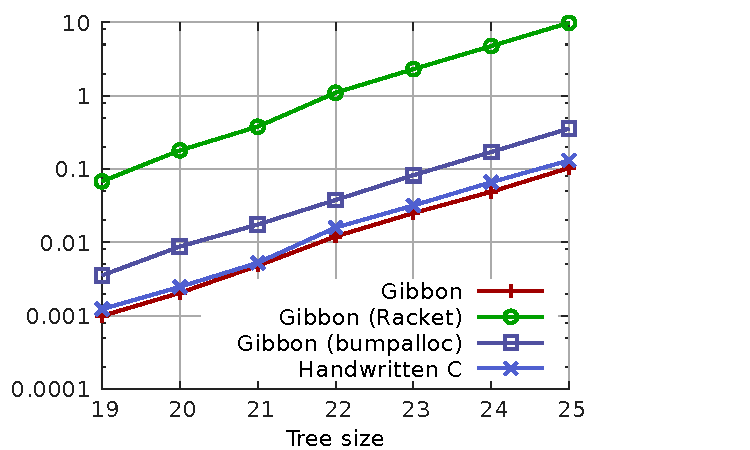
\includegraphics[width=2.9in]{./figs/shootout_buildtree.pdf}    
%    \label{fig:}
  \end{minipage}
  $ $ 
  \begin{minipage}{.32\textwidth}
    \hspace{-4mm}
    \hspace{2mm}
    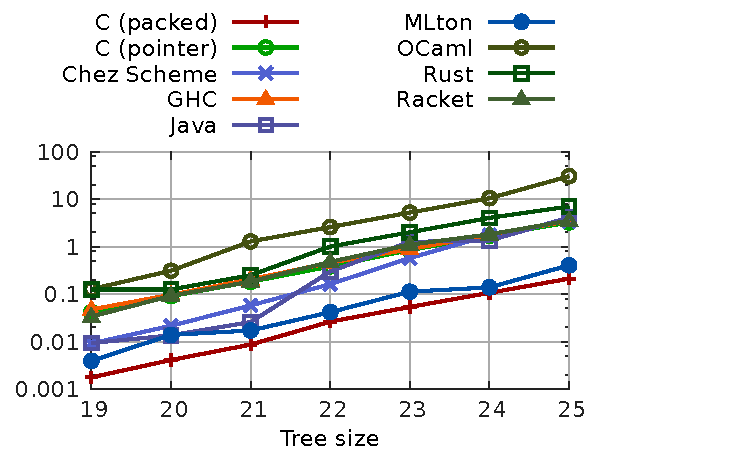
\includegraphics[width=2.9in]{./figs/shootout_add1.pdf}
%    \label{fig:}
  \end{minipage}
  $ $
  \begin{minipage}{.32\textwidth}
    \centering
        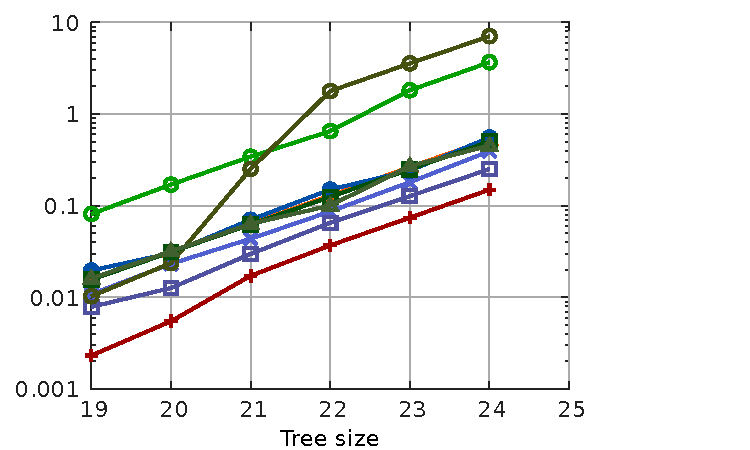
\includegraphics[width=2.9in]{./figs/shootout_sumtree.pdf}
%    \label{fig:}
  \end{minipage}

\end{minipage}
  \vspace{-3mm}
  \caption{Performance when building, mapping add1, and summing a tree respectively.
    Traditional compiler approaches vs. the packed approach.  All handwritten
    implementations.  X axis is tree {\em depth}, implying $2^N$ leaves.  Y axis
  shows time in seconds.}
  \label{fig:shootout1}
\end{figure}

\begin{figure}[t]
  \vspace{-2mm}
\begin{minipage}{1.04\textwidth}
  \begin{minipage}{.49\textwidth}
    \centering
    %   \includegraphics[width=\textwidth]{./figs/.pdf}
    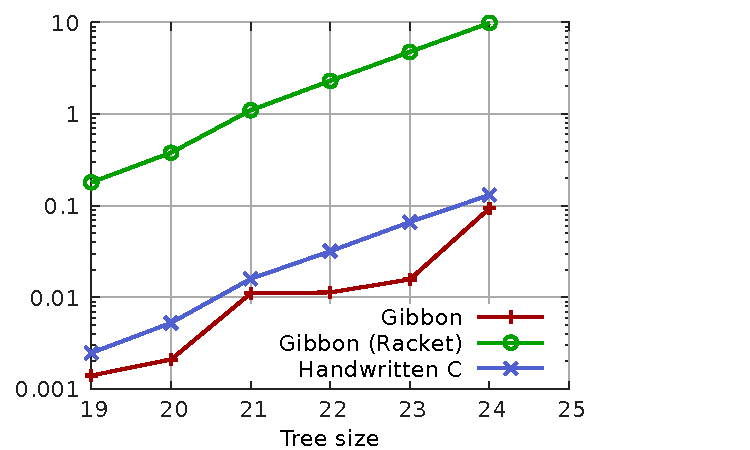
\includegraphics[width=3.8in]{./figs/shootout_gibbon_buildtree.pdf}
%    \label{fig:}
  \end{minipage}
  %  \hspace{0.1\textwidth}
  $ $ 
  \begin{minipage}{.49\textwidth}
    \centering
    %   \includegraphics[width=\textwidth]{./figs/.pdf}
    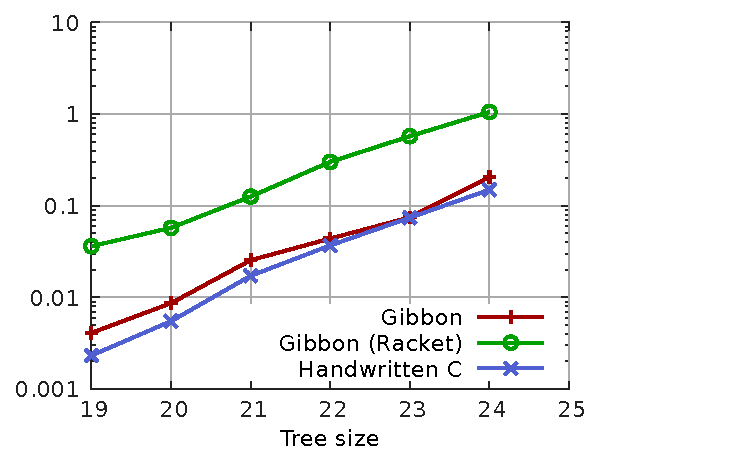
\includegraphics[width=3.8in]{./figs/shootout_gibbon_sumtree.pdf}
%    \label{fig:}
  \end{minipage}
\end{minipage}
   \vspace{-4mm}
   \caption{Cursor-inserting compiler---performance compared to handwritten C
     implementation.  Tree building (left) and tree summing (right). The Gibbon
     prototype is currently embedded in Racket, so we show its Racket backend as
   well.}
   \label{fig:shootout2}
   \vspace{-4mm}
\end{figure}


\begin{figure}[t]
  \vspace{-5mm}
\begin{minipage}{1.04\textwidth}
  \begin{minipage}{.49\textwidth}
    \centering
    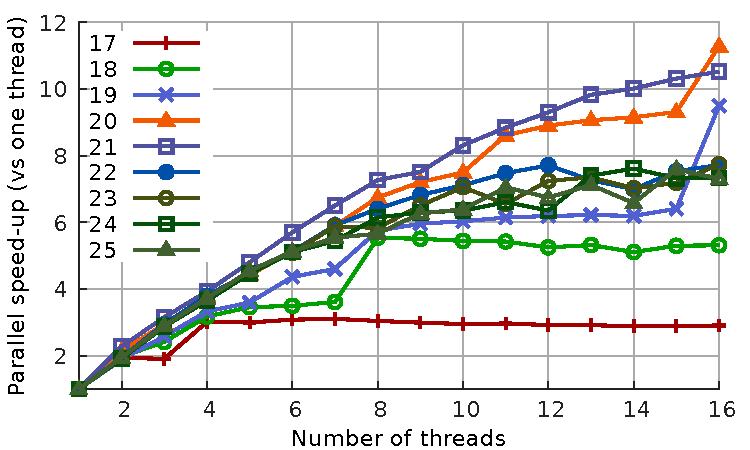
\includegraphics[width=\textwidth]{./figs/speedup_cilk.pdf}
%    \label{fig:}
  \end{minipage}
  %  \hspace{0.1\textwidth}
  $ $ 
  \begin{minipage}{.49\textwidth}
    \centering
    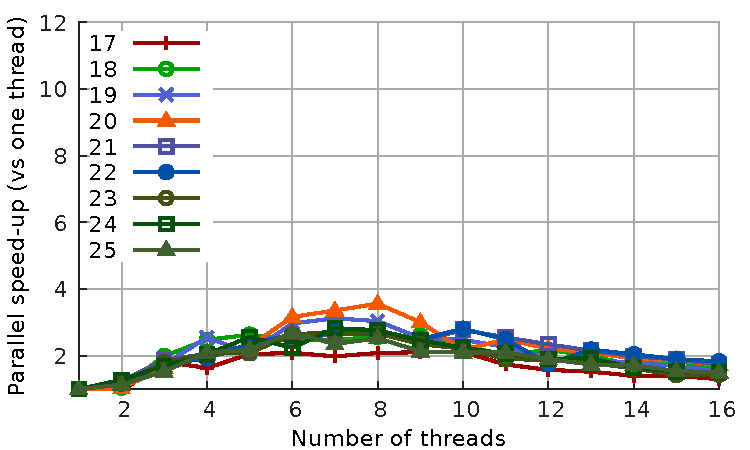
\includegraphics[width=\textwidth]{./figs/speedup_ghc.pdf}
    % \includegraphics[width=60mm]{example-image-b}
%    \label{fig:}
  \end{minipage}
\end{minipage}
   \caption{Parallel speedup: mapping a function over a packed tree.  This
     compares a Cilk (C) implementation using the packed with layout information
     that allows random access to subtrees (left).  For comparison, we also show
     the parallel speedup from a mature parallel functional compiler (GHC,
     right).  All lines are normalized to their own 1-core speeds.  In absolute
     terms, GHC starts off 34$\times$ slower than our approach at one core, and
     grows to 223$\times$ slower at 16 cores.}
   \label{fig:shootout}
      \vspace{-4mm}
\end{figure}
% C/1 0.0036089296875
% HS/1 0.1226078125,
% (/ 0.1226078125 0.0036089296875 ) 34 times

% C/16    0.000319918212890625
% HS/16   0.07138175
% (/ 0.07138175 0.000319918212890625) 223 times


% ================================================================================
\section{Implementation}
% ================================================================================

\note{Current prototype implementation, status}



% ================================================================================
\section{Evaluation}
% ================================================================================

We evaluate the performance of our approach in four ways. First, we
demonstrate via small microbenchmarks that packed data representation
provides significant performance wins across a variety of
languages---including languages with good performance on pointer-based
traversals---and that our compiler produces code competetive with any
existing system. Second, we build several standard compiler passes
operating on Racket's intermediate representation, and show
substantial speedup operating on inputs gathered from existing Racket
programs. Third, we build a type checker for a small language, and
benchmark it on large synthetic inputs, demonstrating significant
speedup for a more complex and data-heavy workload. Fourth, we
implement a point-correlation benchmark using a kd-tree, again showing
major performance benefits for packed representations. Additionally,
we \note{something something parallel}

All benchmarks were conducted on a \dots.

\subsection{Microbenchmarks}
% ----------------------------------------

Our first benchmarks return to the example from section 2,
manipulating simple binary trees. We implement 3 operations:
constructing a tree, incrementing the values in a tree, and summing
the elements of a tree. To understand the performance of packed data
representations, we implemented these three operations in multiple
ways across a variety of languages: with pointer-based trees in
Racket, Chez Scheme, MLton, GHC Haskell, and C (using both \texttt{malloc} as well
as a fast bump-pointer allocator). We also implemented packed versions
using handwritten C code similar to that of section 2, as well as a
packed version in Racket. Finally, we implemented the benchmark in
\treelang{}, and executed it using both the simple Racket backend and
the optimizing backend that is the focus of this paper.

The results show a clear win for packed representations, in some cases
with 100x speedup over pointer-based representations in
garbage-collected languages. Further, our compiler-generated code is
competetive with handwritten C for packed data.

%\note{A ``language shootout'' of add1-tree benchmarks.}


\subsection{Compiler passes on realistic inputs}
% --------------------------------------------

\note{Racket core AST benchmarks}


\subsection{Typechecking benchmark}
% --------------------------------------------

\note{type check the simply-typed $\lambda$ calculus in \treelang{}}

\subsection{Point correlation}
% --------------------------------------------
Point correlation  is a well-known algorithm that is used in data mining\cite{gray2000n},
given a set of points in a k-dimensional space, point correlation computes the number of points in the space  that lies within a
distance r from a given point p, one efficient way of searching such spaces is to store them in  kd-trees \cite{gray2000n}. 

A kd-tree is a binary space partitioning tree that in its simplest form  splits the space at each internal node into two sub-spaces
around a split axes in one of the space dimensions, the left subtree stores the points to the left of the split access
and the right subtree sotres the points to the right of the split access, the split axes alternates between the dimensions of
the space at each level of the tree, when the number of the points in the subtree is one, a leaf node that stores
that point is constructed.


In a naive implementation of point correlation each point in the space need to be checked, however kd-trees 
allow the search process to skip some regions in the space ;by storing at each internal node the boundaries within which all descendent points lies,
and use that information to skip a subtree if the given point is far enough from the boundaries.

Unlike the rest of the benchmarks, point correlation does not necessary traverse the whole tree due to the early trucation condition,
this requires an additional pointer to be stored at each internal node  as discussed earlier, this pointer will be read if an early truncation occur to redirect the traversal to the
next node to be visited.

  
\begin{figure}[htp]
\begin{minipage}{1.04\textwidth}
  \begin{minipage}{.49\textwidth}
    \centering
    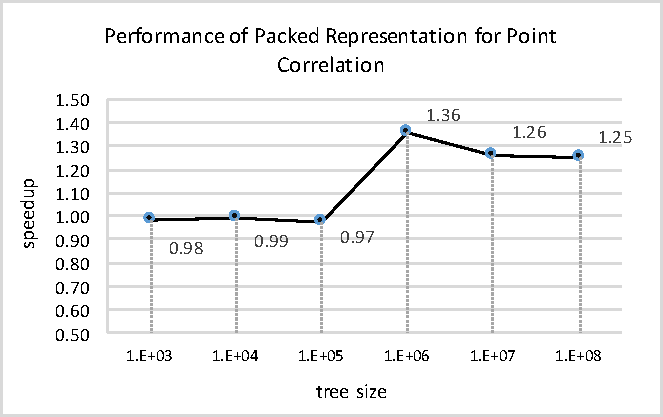
\includegraphics[width=\textwidth]{./figs/pointCorr_perf.pdf}

  \end{minipage}
  $ $ 
  \begin{minipage}{.49\textwidth}
    \centering
    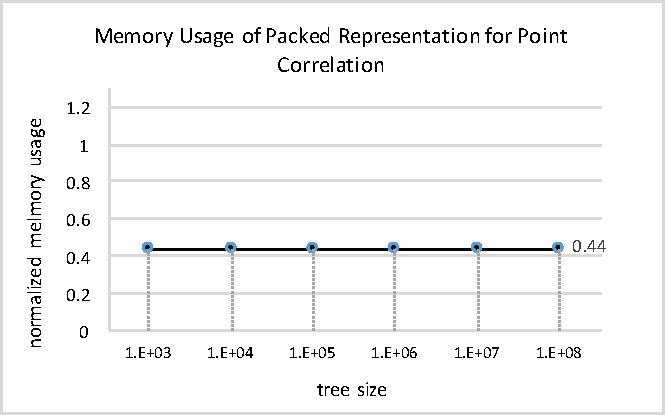
\includegraphics[width=\textwidth]{./figs/pointCorr_MemUsage.pdf}
    % \includegraphics[width=60mm]{example-image-b}
%    \label{fig:}

  \end{minipage}
\end{minipage}
   \caption{normalized runtime performance and memory usage of packed point correlation with respect pointer based implementation }
         \label{fig:pointCorr}
\end{figure}

  
Figure \ref{fig:pointCorr} shows the speedup and the memory usage of the  packed version  with respect to the standard pointer based implementation for different tree sizes,
packed representation uses 56\% less memory to represents the the tree than the pointer based representation, this reduction in memory usage has two sources;
the elimination of the left child pointer and the elimination of the gaps between the structure data members that are added by default for memory alignment purposes.
The runtime performance of the packed version is almost the same as the pointer based for small trees, however when the size of the tree is large enough the packed version 
shows up to 35\% speed up.



\subsection{Parallelism opportunity study}
% --------------------------------------------

\note{Report preliminary parallel microbenchmark results, showing the potential
  for future work here.}




% ================================================================================
\section{Future work}
% ================================================================================

\note{Data type factoring, storing leaves in a separate, dense, aligned vector.
This enables (1) vectorization of numeric operations, and (2) separating
out pointers that the GC must traverse.  This can prove essential for an
open-world implementation in a managed language.}


\note{A large space of parallelism design choices.}

\note{}


%% % ================================================================================
%% \appendix
%% \section{Appendix Title}
%% % ================================================================================

%% This is the text of the appendix, if you need one.

%% \acks

%% Acknowledgments, if needed.

% \bibliographystyle{abbrvnat}
\bibliographystyle{abbrv}

% If you can't commit to the submodule right this second, just copy
% this file to ./refs.bib :
\bibliography{bibs/refs}

% The bibliography should be embedded for final submission.
%% \begin{thebibliography}{}
%% \softraggedright
%% \bibitem[Smith et~al.(2009)Smith, Jones]{smith02}
%% P. Q. Smith, and X. Y. Jones. ...reference text...
%% \end{thebibliography}


\end{document}


